%% Copyright (C) 2021 Alessandro Clerici Lorenzini
%
% This work may be distributed and/or modified under the
% conditions of the LaTeX Project Public License, either version 1.3
% of this license or (at your option) any later version.
% The latest version of this license is in
%   http://www.latex-project.org/lppl.txt
% and version 1.3 or later is part of all distributions of LaTeX
% version 2005/12/01 or later.
%
% This work has the LPPL maintenance status `maintained'.
%
% The Current Maintainer of this work is Alessandro Clerici Lorenzini
%
% This work consists of the files listed in work.txt

\graphicspath{ {./images/} } 	




\section{Statistica descrittiva}
\begin{itemize}
\item Popolazione: insieme di tutti gli elementi che ci interessano
\item Campione: sottoinsieme (rappresentativo) della popolazione che viene studiato:\\
		- Un campione casuale è considerato se i membri sono i scelti in modo tale che tutte le possibili scelte dei $k$ membri siano equiprobabili\\
		- Un campione casuale è chiamato stratificato se sono necessarie più informazioni iniziali
\item Frequenza assoluta ($f$): numero di occorrenza di un dato valore in un esperimento
\item Frequenza relativa: $\frac{f}{n}$ ove $f$ rappresenta la frequenza, ed $n$ il numero totale
\end{itemize}

\subsection{Tabelle e grafici}
Quando i valori distinti sono pochi è giusto applicabile grafici a bastoncini, grafici poligonali ed il grafico a barre. Quando il numero di valori è alto, li suddividiamo in range distinti e li organizziamo sugli istogrammi di frequenze, o istogrammi di frequenze relative.

\subsection{Media, mediana, moda}
Una serie di analisi preliminari che possiamo fare su un campione sono la \emph{media, mediana, e la moda}, che chiameremo \emph{campionaria}. 

Riguardo al nostro campione diciamo che $n$ rappresenta la dimensione, o taglia del campione; mentre ${\{x_1, ..., x_n\}}$ rappresentano gli insiemi del nostro campione.
\begin{itemize}
\item La media campionaria rappresenta la media aritmetica, e rappresenta l'operatore lineare. %Manca la definizione, prendi da pagina 1, nozione di frequenza relativa, 3 modalità totali per il calcolo della media campionaria
\item La mediana campionaria rappresenta una stima \emph{più robusta} della media campionaria (esempio patente), l'outlier o valore fuori scala, rappresenta un valore del campione che pesa in maniera negativa sulla nostra stima. 

La mediana campionaria è uno stimatore "robusto" rispetto agli outlier; viene calcolato riordinando i valori in ordine di grandezza, e prendendo il valore/valori centrali. %Guardare su foglio 1R, definizione, calcolo
\item La moda campionaria rappresenta il valore con frequenza massima
\end{itemize}

\subsection{Concetto di dispersione e varianza campionaria}
Consideriamo due insiemi con una dispersione di carattere molto diverso, ad esempio\begin{center}
$A = \{1, 2, 5, 6, 7\}$ \quad \={a}  = 4\\
$B = \{-40, 0, 5, 20, 35\}$ \quad \={b}  = 4\\
\end{center}
E' verificabile che la media campionaria di questi insiemi è la medesima, ma hanno un carattere di dispersione molto differente. Come possiamo rappresentare questo concetto? 
Un modo preliminare è quello di considerare gli scarti dei valori, rispetto ad un valore centrale che può essere ad esempio la media campionaria. 

Viene tuttavia intuitivo che che la somma degli scarti risulta sempre uguale a 0, sommando e sottraendo gli scarti totali non ci restituisce niente, possiamo tuttavia considerare gli scarti indipendentemente dal segno. Quello che utilizziamo è quindi il valore assoluto degli scarti, consideriamo quindi il quadrato (gestire il valore assoluto è difficile).

\subsubsection{La varianza campionaria}

Introduciamo quindi la \textbf{varianza campionaria} rappresentato dalla dicitura $s^2$. 
ed è definita come:
\begin{equation*}
s^2 = \frac{\sum_{i=1}^n (x_i - \text{\={x}}) ^2 }{n-1}
\end{equation*}
%manca la formula qua (09/03_1)

Di conseguenza calcolando la radice ricaviamo: $s = \sqrt{s^2}$ chiamata \textbf{deviazione standard campionaria}. 
\subsubsection{Scalatura e traslazione}
Come viene influenzata la deviazione standard campionaria rispetto alla scalatura e rispetto alla traslazione? 

Se moltiplichiamo ciascun valore per una costante $c$, per ottenere un nuovo insieme
\begin{equation*}
y_i = cx_i \qquad i = 1, .. , n
\end{equation*}
La varianza campionaria dei valori $y$ è uguale alla varianza campionaria dei valori $x$ moltiplicata per $c^2$ ovvero:
\begin{equation*}
s^2_y = c^2s^2_x
\end{equation*}

Rispetto alla \textbf{scalatura (elevamento a potenza)} la nuova deviazione standard diventa
\begin{center}
$a^2s^2x$\\
ove $x$ è generalizzabile come l'insieme dei vecchi valori
\end{center}
Se prendiamo un insieme, ed eleviamo a potenza i valori all'interno, la nuova deviazione è strettamente legata al valore della deviazione standard campionaria iniziale.

Rispetto alla \textbf{traslazione (spostamento consistente per tutti i campioni)} la deviazione standard rimane costante. Viene intuitivo che dato un insieme, se traslazione di $n$ tutti gli elementi, la deviazione tra loro rimane costante.

\subsection{Mediana campionaria}
La mediana, come abbiamo detto, rappresenta il valore centrale di un insieme dopo un riordinamento. Possiamo tuttavia estendere questo concetto con il seguente enunciato:
Il valore della mediana campionaria è il valore che \begin{itemize}
\item minore o uguale del $50\%$ dei dati
\item maggiore o uguale del $50\%$ dei dati
\end{itemize}
Possiamo estendere il concetto di mediana manipolando il valore in \% che vogliamo, in particolare stiamo parlando di quantile. 
\subsection{Quantile campionario}
Il quantile campionario rappresenta la generalizzazione della mediana. In particolare può essere utilizzato per trovare il valore del campione che è maggiore o uguale dell'$i_{esimo}$ valore dei campioni. 

Consideriamo un campione di $n = 20$ elementi, e un $q = 0,95$. Vogliamo quindi trovare il valore che è maggiore o uguale di $20 * 0,95 = 19$ elementi e minore o uguale $n - q = 1$ elementi. Se l'intersezione è rappresentata da due valori possiamo fare la somma e la divisione tra due.\\

Possiamo estendere ulteriormente il concetto di quantile con i \emph{quartili} (0-4), \emph{percentili} (0-100), \emph{decili} (0-10) in base al tipo di unità di misura che vogliamo utilizzare.

\subsubsection{Box Plot} 
E' una rappresentazione grafica che riassume le principali caratteristiche di un campione di dati. Tale rappresentazione contiene due componenti principali:
\begin{itemize}
\item una scatola, intesa come un rettangolo che evidenzia il primo e il terzo quartile campionario dei dati, che corrispondono alle due basi, e la mediana, indicata tramite un segmento parallelo alle basi stesse;
\item due baffi, che si estendono dagli estremi della scatola fino a raggiungere il minimo e il massimo valore osservato.
\end{itemize}
Il box è definito dal range interquantile, dato dalla differenza fra il III e il I quantile.

\subsubsection{QQ Plot} 

E' una rappresentazione grafica che considera due campioni al fine di valutare la validità dell’ipotesi che i campioni stessi seguano una medesima distribuzione. Questi diagrammi si basano sul fatto (che non dimostreremo) che i quantili campionari rappresentano l’approssimazione di quantili teorici che, considerati tutti insieme, individuano univocamente la distribuzione dei dati.

Pertanto, se due campioni hanno un’uguale distribuzione, allora estraendo da entrambi il quantile di un livello fissato si dovranno ottenere due numeri molto vicini (in quanto essi rappresentano approssimazioni diverse di uno stesso valore).


\subsubsection{Gli insiemi di dati normali e la regola empirica}
Molti grandi insiemi hanno istogrammi dall'aspetto simile, sono infatti simmetrici al punto con frequenza massima, e assumono una forma a campana intorno. Questi insiemi sono chiamati \emph{normali}. Rispetto agli insiemi di dati normali con media campionaria \={x} e deviazione standard campionaria $s$ possiamo dire:
\begin{enumerate}
\item approssimativamente 68\% delle osservazioni rientrano nell'intervallo \={x}$ \pm s$
\item approssimativamente 95\% delle osservazioni rientrano nell'intervallo \={x}$ \pm 2s$
\item approssimativamente 99.7\% delle osservazioni rientrano nell'intervallo \={x}$ \pm 3s$
\end{enumerate}



\section{Campione a coppie}
Consideriamo un dataset formato da due attributi per ogni campione, come andiamo a gestire questo tipo di dati?
\begin{equation*}
		x_1, ..., x_n \quad e  \quad y_1, ..., y_n
	\end{equation*}
	L'insieme delle coppie sarà la seguente:
\begin{equation*}
		{(x_1, y_1), ..., (x_n, y_n)}
	\end{equation*}
\subsection{Il diagramma di dispersione}
O \emph{scatter plot}, è utilizzabile per rappresentare gli elementi del campione su un piano cartesiano. %x, y -> per rappresentare sul piano 

Quando \emph{tendenzialmente} i valori delle osservazioni di un valore $x$ ed un valore $y$ sono siamo nel caso di una relazione di tipo diretta. Basandoci sulla relazione tra i valori possiamo identificare una funzione lineare (o non) con la quale approssimare una ipotetica immagine, dato un valore. 

\subsection{Covarianza campionaria}
%Pagina 3.1
Come possiamo definire matematicamente se un campione è "piccolo" o "grande", essendo queste assunzioni di carattere oggettivo? 

Utilizziamo la covarianza campionaria (sempre basata sulla media campionaria) per calcolare un indice numerico per un'interpretazione oggettiva. Se la covarianza campionaria ha un valore positivo, allora la relazione è diretta, in maniera inversa se la covarianza campionaria ha un valore negativo, allora la relazione è indiretta (bisogna tuttavia accennare che la covarianza campionaria non è un indice robusto rispetto agli outlier).

\subsection{Indice di correlazione lineare}
A partire dalla covarianza campionaria è possibile ottenere l'indice di correlazione lineare (spesso denominato come r), dividendolo per le varianze campionaria dei due campioni. Il segno dell'indice di correlazione lineare è sempre uguale al segno dell'indice di covarianza campionaria. Questo indice avrà sempre un valore:
\begin{equation*}
		-1 \leq r \leq 1
	\end{equation*}
	e la sua formula è :
	\begin{align*}
	r & = \frac{	\sum_{i=1}^{n}	 (x_i - \text{\={x}}	)(y_i - \text{ \={y}}	)}{(n-1)s_xs_y}\\
		& = \frac{	\sum_{i=1}^{n} 	(x_i - \text{\={x}}	)(y_i - \text{ \={y}}	)}  {\sqrt{ \sum_{i=1}^n (x_i - \text{\={x}}	)^2 \sum_{i=1}^n (y_i - \text{\={y}})^2  }}
	\end{align*}
	Quando $r > 0$ si dice che i dati sono correlati positivamente, invece quando $r < 0$ si dice che sono correlati negativamente.
Esiste anche una formula alternativa per il calcolo del coefficiente di relazione ovvero: %3 pagina retro

\begin{equation*}
r = \frac{	\sum_{i=1}^n x_iy_i - n \text{\={x}\={y}}}{\sqrt{(\sum_{i=1}^n x_i^2 - n\text{\={x}}^2)(\sum_{i=1}^n y_i^2 - n\text{\={y}}^2)}}
\end{equation*}

\subsection{Eterogeneità e Omogeneità}
Gli indici di eterogeneità e omogeneità vanno a studiare la diversità dei campioni, basandosi sulle frequenze.
\subsection{Indice di Gini (per l'eterogeneità)}
Solitamente indicato con $I$ maiuscolo (invece che minuscolo), e viene formalizzato nel seguente modo:
\begin{equation*}
I = 1 - \sum_{i=1}^m f_j^2
\end{equation*}
Considerando una serie di valori osservabili $v_1, ... v_m$ e una serie di frequenze relative $f_1, ... f_m$.
L'indice di Gini non è mai uguale a 1, e non è mai minore di zero. Possiamo quindi dire che:
\begin{equation*}
0 \leq I < 1
\end{equation*}
In caso di eterogeneità massima (diversità massima) l'indice di Gini è uguale a \begin{equation*}
I = 1
\end{equation*}
Nel caso di omogeneità massima (diversità minima) l'indice di Gini è uguale a 
\begin{equation*}
I = 0
\end{equation*}
L'indice di Gini normalizzato permette all'indice di Gini di includere pure il valore 1, ed rappresentato da
\begin{equation*}
I' = \frac{k}{k-1}I
\end{equation*}
Con il valore di $I'$ che può assumere quindi i seguenti valori:
\begin{equation*}
0 \leq I' \leq 1
\end{equation*}
Questo è preferibile in quanto in precedenza il valore di Gini non poteva mai assumere il valore 1 (massima eterogeneità).

\subsection{Entropia}
Rappresentata dalla lettera H maiuscola ed è definito nel seguente modo:
\begin{equation*}
H = \sum_{j=1}^m f_jlog\frac{1}{f_j} = - \sum_{i=1}^s f_i log f_i
\end{equation*}
$H$ può assumere solo valori $\geq 0 $, i casi particolari sono:
\begin{itemize}
\item caso di omogeneità massima con $H = 0$ %sse $\forall j H_j = 0$ e $\forall_j f_j = 0$ OR $f_j = 1$ 
\item caso di eterogeneità massima con $H = log m $ %sse $ \forall j = f_j = \frac{1}{m}$ e $H = \sum_{j=1}^m f_jlog\frac{1}{m} = log m$
\end{itemize}

\subsection{Concentrazione}
In presenza di variabili che rappresentano beni condivisibili in una popolazione, è possibile chiedersi quanto concentrato il bene sia sulla popolazione.
Consideriamo $n$ osservazioni $a_1, a_2, ..., a_n$, ordinate: 
\begin{equation*}
\text{Valore medio: \={a}} = \frac{1}{n} \sum_i a_i \quad e \quad TOT = n\text{\={a}} = \sum_i a_i
\end{equation*}
\begin{itemize}
\item La concentrazione massima è rappresentata da: $ a_1 = 0, ..., a_{n-1} = 0, a_n = n $ \={a} 
\item La concentrazione minima è rappresentata da: $a_1 = a_2 = a_n =$ \={a}
\item Le frequenze cumulate relative sono rappresentate da $F_i = \frac{i}{n}$
\item Le quantità cumulate relative sono rappresentate da $Q_i = \frac{1}{tot} \sum_{k=1}^i a_k$ (fino all'i-esima osservazione)
\end{itemize}
Su questi indicatori possiamo dire sicuramente che:\\
- I valori $F_i$ e $Q_i$ sono sempre compresi tra 0 e 1: $0 \leq F_i, q_i \leq 1$  \\
- Quando le osservazioni sono ordinate in modo crescente: $Q_i \leq F_i \forall i$ \\
- Quando $F_n$ è uguale ad uno, anche $Q_n$ è uguale ad 1: $Q_n = F_n = 1$

\subsubsection{La curva di Lorentz}
L'area compresa tra la curva dei punti (detta curva di Lorentz) e la retta di equidistribuzione (la retta a 45°) è detta area di concentrazione e può essere utilizzata come base per la definizione di appositi rapporti di concentrazione, di cui l'indice di Gini costituisce un esempio. Maggiore infatti è la concentrazione osservata, maggiore sarà tale area.

\subsection{Trasformazione dei dati}
Consideriamo una serie di osservazioni $x_1, ..., x_m$, abbiamo già visto durante il corso la traslazione e la scalatura.
Consideriamo una funzione $g$ iniettiva:\begin{center}
$g: x \rightarrow x'$
\end{center}
\subsubsection{Traslazione}
\begin{center}
$k > 0$ $g(x) = x + k, g(x) = x-k$
\end{center}
- Gli indici di media, mediana, moda, quantili vengono traslati della stessa quantità $k$\\
- Gli indici di range, distanza interquantile, varianza e deviazione rimangono invariati.
\subsubsection{Scalatura}
\begin{center}
$h \neq 0$ $g(x) = \frac{x}{h}$
\end{center}
- Gli indici di media, mediana, quantili, range di variazione, distanza interquantile e deviazione standard vengono scalati di $\frac{1}{h}$\\
- L'indice di varianza viene scalato di $\frac{1}{h^2}$ mentre la deviazione standard viene scalata di $\frac{1}{h}$

\subsubsection{Cambiamento di scala e di origine}
Se abbiamo dei valori nell'intervallo di $[a, b]$, e vogliamo adattarli all'intervallo $[c, d]$, ovvero: 
\begin{center}
$(a, b) \rightarrow (c, d)$
\end{center}
La trasformazione che applichiamo è la seguente \begin{center}
$\frac{x'-c}{d-c} = \frac{x-a}{b-a}$
\end{center}
Che può essere semplificato nel seguente modo:
\begin{center}
$x' = c + \frac{d-c}{b-a} (x-a)$
\end{center}
Consideriamo le seguenti particolare mappature:
\begin{itemize}
\item $(a, b) \rightarrow (0,1): x' = \frac{x-a}{b-a}$
\item $(a, b) \rightarrow (-1, +1): x' = 2 \frac{x-a}{b-a} -1$
\end{itemize}

\subsubsection{Standardizzazione}
O normalizzazione rappresenta un caso particolare di cambiamento di origine e scala, e consiste nell'applicare una scala il cui fattore è uguale alla deviazione standard dei valori, per poi traslare verso sinistra rispetto alla media dei valori. Con media campionaria \={x} e deviazione standard campionaria $\sigma_x$, la trasformazione sarà:
\begin{equation*}
	x \rightarrow x' = \frac{x-\text{\={x}}}{\sigma_o}
\end{equation*}  
La trasformazione di standardizzazione trasforma pertanto l'insieme dei valori in un altro insieme di valori la cui media è 0 e la cui varianza è 1.



\subsubsection{Trasformazione logaritmica}
Quando i valori di una variabile osservata sono molto grandi oppure molto distanziati, conviene pensare a tali valori come potenza di una data base, ragionando in termini del relativo esponente.
\begin{center}
$g(x) = log x$
\end{center}

\subsection{ANOVA - Analysis of variance}
Anova, o analysis of variance viene impiegato quando dato un insieme di osservazione, è possibile suddividerli in $G$ gruppi diversi. L'idea alla base di questo metodo è che se non vi sono sostanziali differenze tra i gruppi considerati, allora calcolare la varianza all'interno di un gruppo qualsiasi non dovrebbe portare a un risultato molto dissimile da quello ottenuto effettuando il calcolo su tutti i dati a disposizione.

Intuitivamente con \begin{center}
$\sum_{i=1}^G n_i = n$
\end{center}
Rappresenta l'insieme di tutte le osservazioni, e
$x_i^g$ rappresenta l'i-esima osservazione del g-esimo gruppo
ove $g = 1, ..., G$ e $n_g =$ \# osservazioni nel g-esimo gruppo
%porca di quella
\begin{center}
 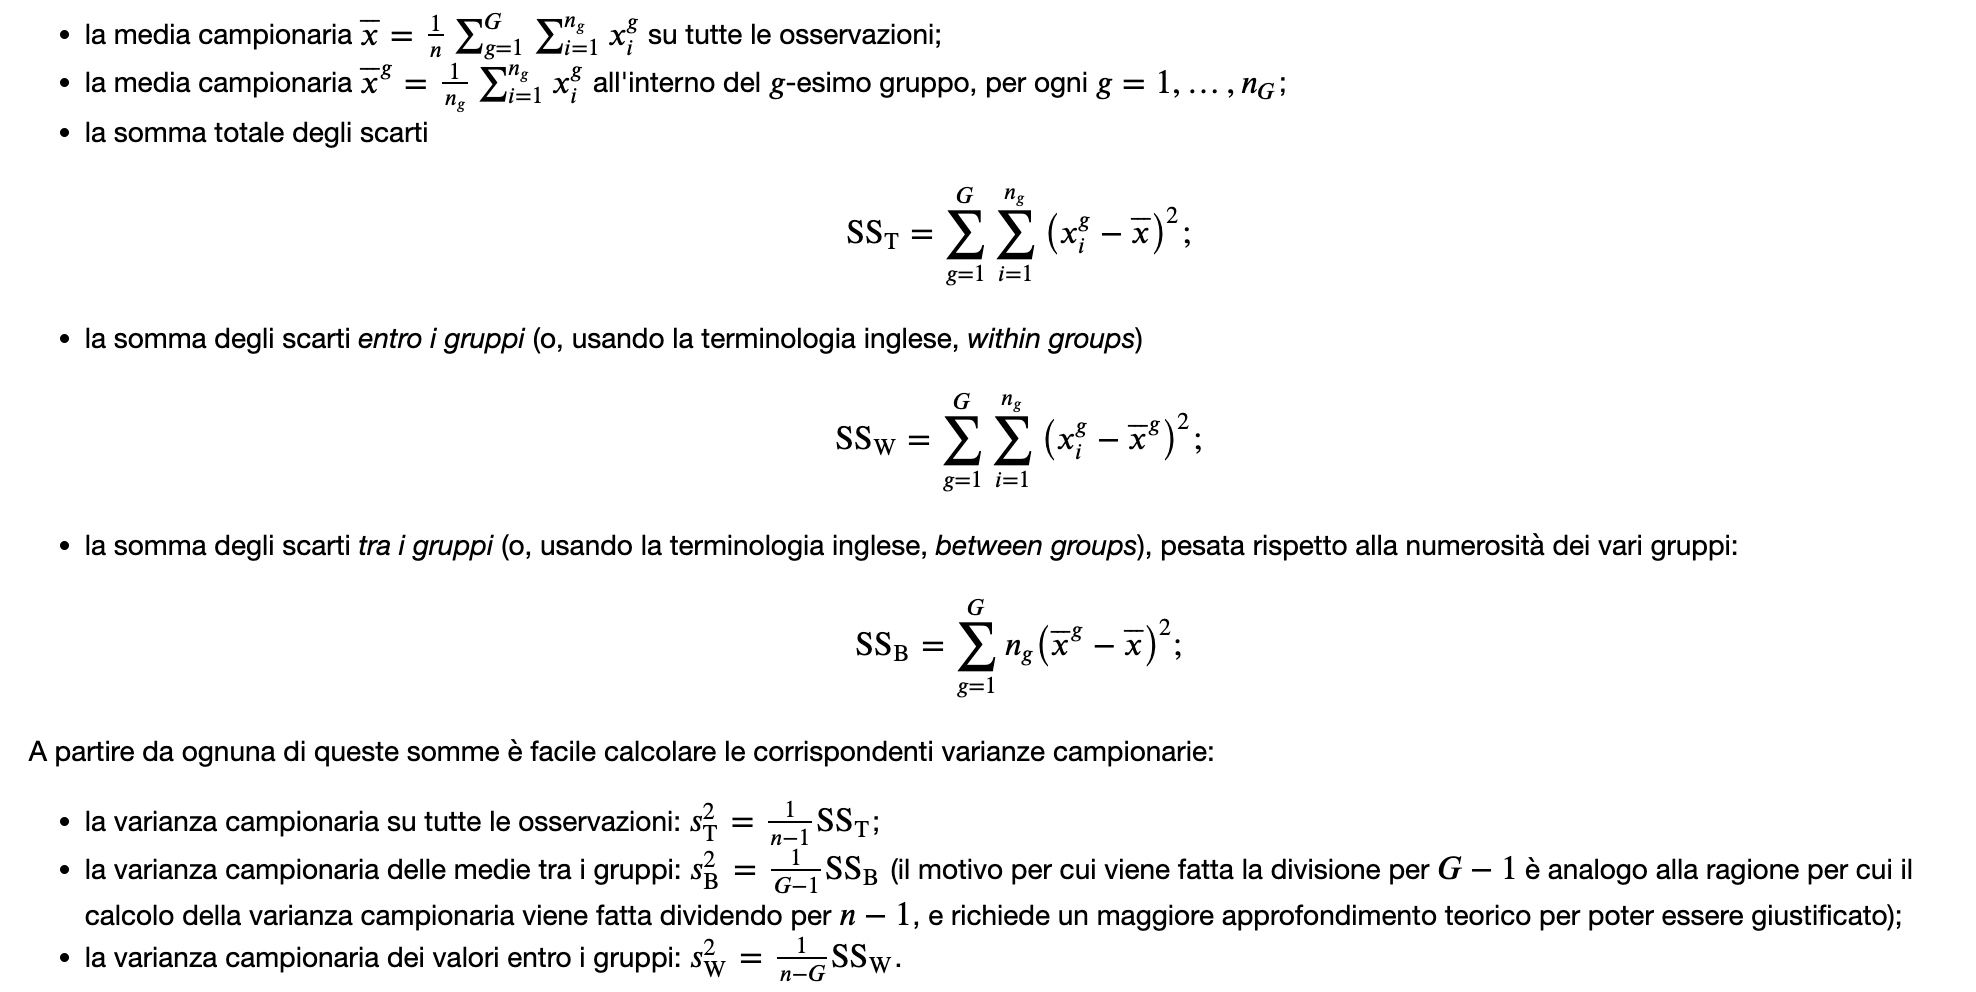
\includegraphics[scale=0.4]{anova.png}
\end{center}


E' possibile dimostrare che\begin{center}
$SS_T = SS_W + SS_B$
\end{center}





\section{Definizioni}
La definizione assiomatica della probabilità riassume in pochi punti quei concetti che si possono definire intuitivi nel calcolo delle probabilità.

\subsection{L'algebra degli eventi}
\begin{defin}
	Scelto un insieme $\Omega$ detto spazio campionario o degli eventi, si dice esito un elemento $\omega\in\Omega$ dell'insieme ed evento un suo sottoinsieme $E\subseteq\Omega$.

\end{defin}
\subsection*{Le proprietà dell'algebra degli eventi}
Utilizzando questi formalismi possiamo definire anche:
\begin{itemize}
\item $E \cup F$ l'insieme degli eventi che sono presenti nell'insieme $E$ o nell'insieme $F$
\item $E \cap F$ l'insieme degli eventi che sono presenti sia nell'insieme $E$ che nell'insieme $F$
\item $\bar E$ rappresenta l'insieme degli eventi complementare, ne consegue che il complementare di $\Omega$ è $\emptyset$, ovvero: $\bar \Omega = \emptyset$
\item Per definizione l'insieme vuoto $\emptyset$ rappresenta un evento, ed è l'evento che non può accadere e/o l'evento impossibile.
\end{itemize}
Bisogna infine accennare che sugli insiemi eventi valgono le proprietà di:
\begin{itemize}
\item Commutatività: $E \cup F = F \cup E$
\item Associatività: $(E \cup F) \cup G = E \cup (F \cup G)$
\item Distributività: $E \cup (F \cap G) = (E \cup F) \cap (E \cup G)$
\item De morgan: $(E \cup F) = (\bar E \cap \bar F)$
\end{itemize}

\begin{defin}
	Sia $\A\in2^\Omega$ una collezione di sottoinsiemi di $\Omega$. Allora $\A$ è un'algebra se
	\begin{align*}
		 & \bullet ~ \Omega\in \A                                                                                            		\\
		 & \bullet ~ \forall E\subseteq\Omega\qquad E\in\A\Rightarrow \bar E\in\A \qquad\text{con }\bar E:=\Omega\setminus E \\
		 & \bullet ~ \forall E_1,\dots E_n\in\Omega\qquad \forall i~E_i\in\A\Rightarrow \bigcup\limits_{i=1}^n E_i \in\A
	\end{align*}
	$\A$ è una $\sigma$-algebra su $\Omega$ se l'ultima condizione si può estendere a unioni numerabili qualsiasi, ovvero se vale anche per $n \rightarrow \infty$.
\end{defin} %1) L'evento certo deve essere contenuto all'interno dell'algebra\\

%2) Se sono in grado di determinare la probabilità di un evento, devo essere in grado di determinare la probabilità anche del suo complementare


\subsection{Assiomi di Kolmogorov}
La probabilità viene definita come una funzione di un'algebra degli eventi $\A$ in $\R$:
\begin{equation*}
	P:\A\to\R
\end{equation*}

I seguenti assiomi, detti di Kolmogorov, decretano le proprietà che la probabilità rispetta:


\subsubsection{Primo assioma}
L'immagine di $P$ è l'insieme $[0,1]\in\R$. Equivalentemente, la probabilità di qualunque evento è compresa tra $0$ e $1$:
\begin{equation*}
	\forall E\in\A\qquad 0\leq P(E)\leq 1
\end{equation*}


\subsubsection{Secondo assioma}
La probabilità dello spazio campionario è $1$:
\begin{equation*}
	P(\Omega)=1
\end{equation*}


\subsubsection{Terzo assioma}
La probabilità dell'unione di eventi mutuamente esclusivi, cioè disgiunti (intuitivamente, l'avvenire dell'uno esclude l'avvenire dell'altro), è uguale alla somma delle probabilità dei singoli:
\begin{equation*}
	\forall E_1,\dots,E_n\in\A\qquad \forall i,j~E_i\cap E_j = \emptyset \Rightarrow P\left( \bigcup_{i=1}^n E_i \right)=\sum_{i=1}^n P(E_i)
\end{equation*}



\subsection{Teoremi elementari}
Dagli assiomi di Kolmogorov derivano alcune proprietà elementari facilmente dimostrabili.


\subsubsection{Probabilità dell'evento complementare}
\begin{defin}
	Dato un evento $E\in\A$, l'evento complementare è l'evento $\bar E := \Omega\setminus E$.
\end{defin}
\begin{teor}[probabilità dell'evento complementare] \label{t:probcompl}
	Dato un evento $E$, se la probabilità di $E$ è $P(E)$, la probabilità dell'evento complementare di $E$ è $1-P(E)$:
	\begin{equation*}
		\forall E\in\A\qquad P(\bar E)=1-P(E)
	\end{equation*}
\end{teor}
\begin{proof}
	\begin{align*}
		  & \left.
		\begin{array}{cc}
			E\cap\bar E=\emptyset \\
			E\cup\bar E=\Omega
		\end{array} \right\}  \bc{definizione di evento complementare} \\
		1 & = P(\Omega)        \bc{secondo assioma}                                  \\
		  & = P(E\cup\bar E)                                                         \\
		  & = P(E)+P(\bar E)   \bc{terzo assioma}
	\end{align*}
	ergo:
	\begin{equation*}
		P(\bar E)=1-P(E) \qedhere
	\end{equation*}
\end{proof}

\subsubsection{Probabilità dell'unione}
\begin{teor} \label{t:probunion}
	Dati due eventi $E,F\in\A$, la probabilità della loro unione è uguale alla somma delle loro probabilità meno la probabilità dell'intersezione:
	\begin{equation*}
		\forall E,F \in\A\qquad P(E\cup F)=P(E)+P(F)-P(E\cap F)
	\end{equation*}
\end{teor}
\begin{proof}
	L'unione degli eventi è scrivibile come l'unione di due insiemi disgiunti:
	\begin{equation*}
		E\cup F=E \cup (\bar E\cap F) \\[1ex]
	\end{equation*}

	Passando alle probabilità:
	\begin{align*}
		P(E\cup F) & = P(E)+P(\bar E\cap F)                                               \\
		           & = P(E)+P(\bar E\cap F)+P(E\cap F)-P(E\cap F)                         \\
		           & = P(E)+P((\bar E\cap F)\cup (E\cap F))-P(E\cap F) \bc{terzo assioma} \\
		           & = P(E)+P(F)-P(E\cap F)                            \qedbc
	\end{align*}
\end{proof}

\subsubsection{Probabilità dell'evento vuoto}
La probabilità dell'evento vuoto ($\emptyset$) è $0$. Un evento con probabilità nulla viene detto evento impossibile.
\begin{equation*}
	P(\emptyset)=0
\end{equation*}

\begin{proof}
	\begin{align*}
		P(\Omega)    & = 1 \bc{secondo assioma}                       \\
		P(\emptyset) & = P(\bar\Omega)                                \\
		             & = 1 - P(\Omega) \bc{teorema \ref{t:probcompl}} \\
		             & = 1 - 1 = 0     \qedbc
	\end{align*}
\end{proof}



\subsection{Spazi di probabilità}
\begin{defin}
	Uno spazio di probabilità è una tripla $(\Omega,\A,P)$ composta da uno spazio campionario $\Omega$, un'algebra degli eventi $\A$ e una funzione di probabilità $P$.
\end{defin}


\subsubsection{Spazi equiprobabili}
\begin{defin}
	Uno spazio è equiprobabile se gli eventi elementari (cioè corrispondenti a singoletti) hanno probabilità costante $p$.
\end{defin}

Un evento elementare è composto da un singolo esito, cioè è un singoletto dell'insieme delle parti dello spazio campionario.
\begin{teor}
	In uno spazio equiprobabile, la probabilità di ogni evento elementare $e$ è uguale al reciproco del numero $n$ degli eventi elementari (che sono ovviamente a due a due disgiunti):
	\begin{equation}
		P(e)=\frac{1}{n}
	\end{equation}
\end{teor}
\begin{proof}
	\begin{align*}
		1=P(\Omega)=P\left( \bigcup_{i=1}^n e_i \right) \bc{secondo assioma} \\
		=\sum_{i=1}^n P(e_i) = np \bc{terzo assioma}                         \\
	\end{align*}
	Ergo:
	\begin{equation*}
		\forall e_i ~ P(e_i)=p=\frac{1}{n} \qedhere
	\end{equation*}
\end{proof}

Gli eventi non elementari possono essere espressi come unione di eventi elementari.
\begin{teor}
	In uno spazio equiprobabile, dato un evento $E=\{e_1,\dots,e_k\}$:
	\begin{equation}
		P(E)=\frac{|E|}{n}
	\end{equation}
\end{teor}
\begin{proof}
	\begin{equation*}
		P(E)= \sum_{i=1}^{|E|} P(e_i) = \frac{|E|}{n} \qedhere
	\end{equation*}
\end{proof}
